\chapter{Project Management}
\label{ch:intro-pm}

%%%%%%%%%%%%%%%%%%%%%%%%%%%%%%%
\section{Project Structure and Responsibilities}

The LBNF Project is charged by Fermilab and DOE to design and construct conventional and technical facilities needed to support the DUNE Collaboration. LBNF is organized as a DOE/Fermilab project incorporating in-kind contributions from international partners. At this time, the major international partner is CERN, the European Organization for Nuclear Research. LBNF works closely with DUNE through several coordinating groups to ensure scientific direction and coordination for executing the LBNF Project such that the requirements of the program are met. 

LBNF works closely with SURF management to coordinate design and construction for the far site conventional facilities for the DUNE far detector. CERN is providing cryogenics equipment and engineering as part of the cryogenics infrastructure at SURF. The design and construction of LBNF is supported by other laboratories and consultants/contractors that provide scientific, engineering, and technical expertise.  A full description of LBNF Project Management is contained in the LBNF/DUNE Project Management Plan\cite{PMP-10770}.

LBNF coordinates with DUNE through regular technical team interactions between the two Projects as well as more formally through the Joint Management Team where day-to-day management coordination occurs, and the Experiment-Facility Interface Group, where major issues regarding interfaces and items affecting both Projects are discussed. In addition, the Projects share common Project Office staff and systems, and include a single, integrated project resource-loaded schedule and configuration management system. 


LBNF consists of two major L2 subprojects, Far Site Facilities and Near Site Facilities, coordinated through a central Project Office located at Fermilab.  Each L2 Project consists of two large L3 subprojects corresponding to the conventional and technical facilities, respectively, at each site. The project organizational structure, which includes leadership from major partners, is shown in Figure~\ref{lbnf-wbs}.


The LBNF Project team consists of members from Fermilab, CERN, South Dakota Science and Technology Authority (SDSTA), and Brookhaven National Laboratory (BNL).  The team, including members of the Project Office as well as the L2 and L3 managers for the individual subprojects, is assembled by the Project Director. The Project team is shown in Figure~\ref{fig:lbnf-org}. 
Line management for environment, safety and health, and quality assurance flows through the Project Director. 

Through their delegated authority and in consultation with major stakeholders, the L2 Project Managers determine which of their lower-tier managers will be Control Account Managers (CAMs) for the Project WBS. L2 and L3 Project Managers are directly responsible for generating and maintaining the cost estimate, schedule, and resource requirements for their subprojects and for meeting the goals of their subprojects within the accepted baseline cost and schedule. 

\begin{cdrfigure}[LBNF Work Breakdown Structure (WBS) to Level 3]{lbnf-wbs}{LBNF Work Breakdown Structure (WBS) to Level 3 (L3)}
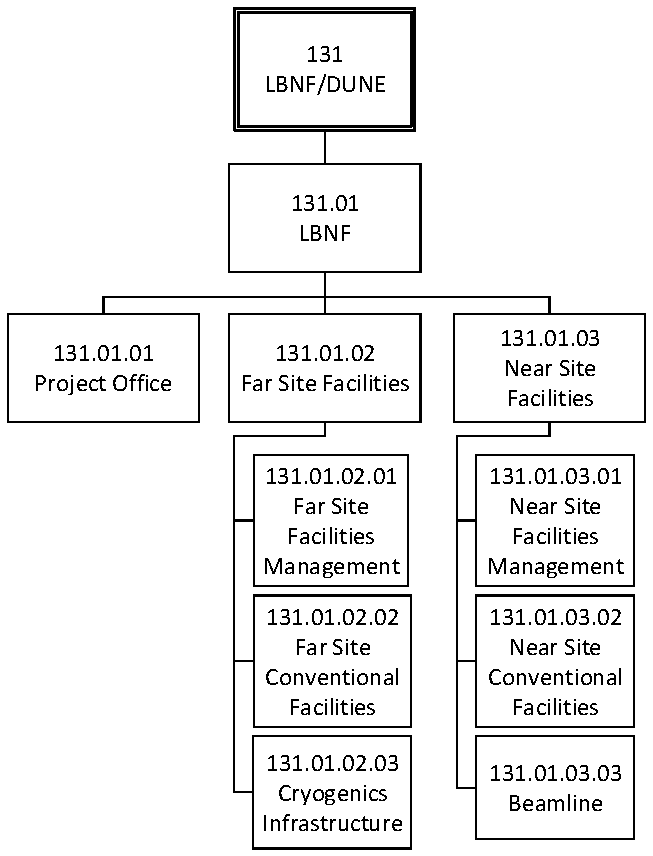
\includegraphics[width=0.6\textwidth]{lbnf-wbs-l3-nonames}
\end{cdrfigure}


\begin{cdrfigure}[LBNF Organization]{lbnf-org}{LBNF Organization}
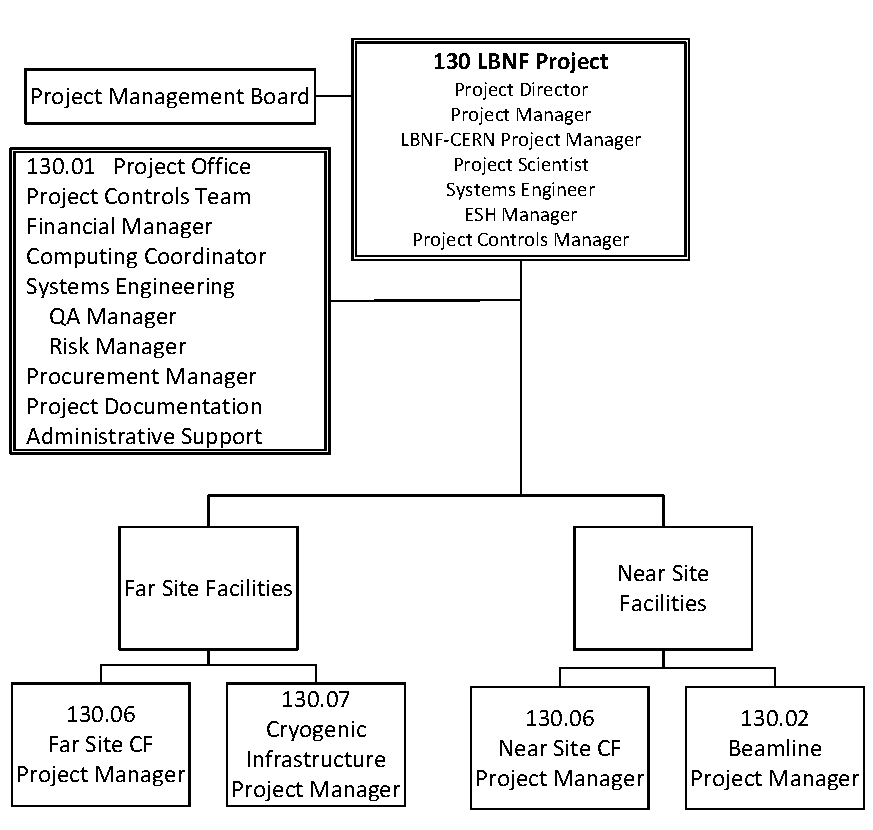
\includegraphics[width=1.0\textwidth, angle=90]{lbnf-org}
\end{cdrfigure}

%%%%%%%%%%%%%%%%%%%%%%%%%%%%%%%
\section{SDSTA and SURF}

LBNF plans to construct facilities at SURF to house and support the DUNE far detector. SURF is owned by the state of South Dakota and managed by the SDSTA. 

Current SURF activities include operations necessary for allowing safe access to the 4850L of the former mine, which houses the existing and under-development science experiments. The DOE is presently funding SDSTA ongoing operations through Lawrence Berkeley National Laboratory (LBNL) and its SURF Operations Office through FY16; starting in FY17 it is expected that this will change, and that funding will flow through Fermilab. 

The LBNF Far Site Facilities Manager is also an employee of SDSTA and is contracted to Fermilab to provide management and coordination of the Far Site Conventional Facilities (CF) and Cryogenics Infrastructure subprojects. LBNF contracts directly with SDSTA for the design of the required CF at SURF; whereas the actual construction of the CF will be directly contracted from Fermilab. Coordination between SDSTA and the LBNF Project is necessary to ensure efficient operations at SURF. This will be facilitated via an agreement between SDSTA and Fermilab (not yet available) that defines responsibilities and methods for working jointly on LBNF Project design and construction. A separate agreement will be written for LBNF Operations. 

%%%%%%%%%%%%%%%%%%%%%%%%%%%%%%%
\section{CERN}

The European Organization for Nuclear Research (CERN) is expected to significantly contribute to LBNF with technical components that are required to support the deployment of both the DUNE detectors and the neutrino beamline. 

%%%%%%%%%%%%%%%%%%%%%%%%%%%%%%%
\section{Coordination within LBNF}

The LBNF Project organization is headed by the LBNF Project Director, who is also the Fermilab Deputy Director for LBNF; this person reports directly to the Fermilab Director. 

Within Fermilab's organization, the LBNF organization includes two new divisions -- Far-Site Facilities and Near-Site Facilities -- as well as a project office, all led by the LBNF Project Director. They have been created to execute the Far Site Facilities and Near Site Facilities subprojects.
The heads of these divisions report to the LBNF Project Manager. 
Any personnel working more than half-time on these subprojects would typically be expected to become a member of one of these divisions, while other contributors will likely be matrixed into part-time roles from other Fermilab Divisions.  The heads of the other Fermilab Divisions work with the L2 and L3 project managers to supply the needed resources on an annual basis.    

The LBNF WBS defines the scope of work. All changes to the WBS must be approved by the LBNF Project Manager prior to implementation.   The current WBS is shown in Figure~\ref{fig:lbnf-wbs}. 
For work on specific tasks required for the LBNF Project at the SURF site, SDSTA assigns engineers and others as required. This is listed in the resource-loaded schedule as contracted work from Fermilab for Far Site CF activities. 
CERN and Fermilab are developing a common cryogenics team to design and produce the Cryogenics Infrastructure subproject deliverables for the far site. CERN provides engineers and other staff as needed to complete their agreed-upon deliverables.  
LBNF has formed several management groups with responsibilities as described below. More detail is provided in the PMP\fixme{add citation, doc 117}.

%\textbf{Project Management Board:} 
LBNF uses a \textit{Project Management Board} to provide formal advice to the Project Director on matters of importance to the LBNF Project as a whole. Such matters include (but are not limited to) those that
\begin{itemize}
\item have significant technical, cost, or schedule impact on the Project
\item have impacts on more than one L2 subproject
\item affect the management systems for the Project
\item have impacts on or result from changes to other Projects on which LBNF is dependent
\item result from external reviews or reviews called by the Project Director
\end{itemize}

The Project Management Board serves as the
\begin{itemize}
\item LBNF Change Control Board, as described in the Configuration Management Plan\cite{CMP-10760} 
\item Risk Management Board, as described in the Fermilab Risk Management Procedure for Projects~\cite{fnal-risk-mgmt} %Plan 
\end{itemize}

%\textbf{FSCF Neutrino Cavity Advisory Board:} 
The Far Site CF (FSCF) Project has engaged three international experts in hard-rock underground construction to advise it periodically through the design and construction process regarding excavation at SURF. This team, the FSCF \textit{Neutrino Cavity Advisory Board (NCAB)}, %The Board 
meets at the request of the FSCF-PM, generally on-site, to discuss specific technical issues. The NCAB produces a report with its findings and conclusions for Project information and action. 

%%%%%%%%%%%%%%%%%%%%%%%%%%%%%%%%%%%%%%%%%%%%%%%%%%%%%
\section{LBNF/DUNE Advisory and Coordinating Structures}
\label{sec:lbnf-dune-interface}

A set of structures has been established to provide coordination among the participating funding agencies, oversight of the LBNF and DUNE projects, and coordination and communication between the two projects.  These structures and the relationships among them are shown in Figure~\ref{fig:lbnfdune-org} and are described in this section.

\begin{cdrfigure}[Joint LBNF/DUNE management structure]{lbnfdune-org}{Joint LBNF/DUNE management structure}
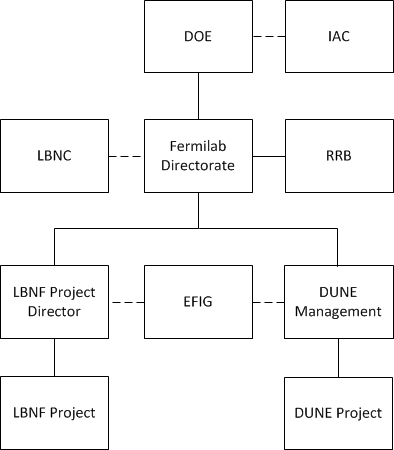
\includegraphics[width=0.8\textwidth]{joint-org}
\end{cdrfigure}

%%%%%%%%%%%%%%%%%%%%%%%%%%%%%%
\subsection{International Advisory Council (IAC) }

The International Advisory Council (IAC) is composed of
regional representatives, such as CERN, and representatives of
funding agencies that make major contributions to LBNF infrastructure or to DUNE. The IAC 
acts as the highest-level international advisory body to the U.S.
DOE and the FNAL Directorate, and facilitates
high-level global coordination across the entire enterprise (LBNF and DUNE).
The IAC is chaired by the DOE Office of Science Associate Director
for High Energy Physics and includes the FNAL Director in its membership.  
The council meets as needed and provides pertinent advice to 
LBNF and DUNE  
through the Fermilab Director.  


Specific responsibilities of the IAC include, but are not limited to,
the following:


\begin{itemize}
\item During the formative stages of LBNF and DUNE
the IAC helps to coordinate the sharing of responsibilities among
the agencies for the construction of LBNF and DUNE.
Individual agency responsibilities for LBNF will be established in
bilateral international agreements with the DOE. Agency contributions to
DUNE will be formalized through separate agreements.

\item The IAC assists in resolving issues, especially those
that cannot be resolved at the Resources Review Boards (RRB) level,
e.g., issues that require substantial redistributions of
responsibilities among the funding agencies.

\item The IAC assists as needed in the coordination,
synthesis and evaluation of input from Project reports charged by
individual funding agencies, LBNF and DUNE Project management,
and/or the IAC itself, leading to recommendations for action by
the managing bodies.
\end{itemize}

The DUNE Co-Spokespersons and/or other participants within
the Fermilab neutrino program will be invited to sessions of the IAC as
needed. Council membership may increase as additional funding agencies
from %certain geographic regions make major contributions to LBNF and DUNE.

%%%%%%%%%%%%%%%%%%%%%%%%%%%%%%
\subsection{Resources Review Boards (RRB)}

The Resources Review Boards (RRB) are composed of representatives from all
funding agencies that sponsor LBNF and DUNE, and from the Fermilab
management. The RRB provides focused monitoring and detailed oversight
of each of the Projects. The Fermilab Director in coordination
with the DUNE RC defines its membership. A representative from the
Fermilab Directorate chairs the boards and
organizes regular meetings to ensure the flow of resources needed
for the smooth progress of the enterprise 
and for its successful completion.  

The managements of the
DUNE Collaboration and the LBNF Project participate in the RRB meetings
and make regular reports to the RRB on technical, managerial,
financial and administrative matters, as well as on status and
progress of the DUNE Collaboration.
DUNE Finance Board members who serve as National Contacts from the 
sponsoring funding agencies will be invited to RRB sessions.

Two groups exist  
within the RRB: RRB-LBNF and RRB-DUNE. Each of
these groups monitors progress and addresses 
 the issues specific to its area 
 while the whole RRB deals with matters
that concern the entire enterprise. 
The RRB meet
biannually; these meetings 
start with a plenary
opening session 
and are followed by 
RRB-LBNF and RRB-DUNE sessions. As DUNE progresses toward
experimental operations, RRB-Computing sessions will convene.


The RRB  employs standing DUNE and LBNF \textit{Scrutiny Groups} as needed
to assist in its responsibilities. The scrutiny groups operate
under the RRB, and provide detailed information on financial and
personnel resources, costing, and other elements under the purview of the RRB.

%Roles 
Responsibilities of the RRB include

\begin{itemize}
\item assisting the DOE and the FNAL Directorate,
with coordinating and developing any required international
agreements between partners
\item monitoring and overseeing the Common Projects and the
use of the Common Funds \fixme{where are these defined?}
\item monitoring and overseeing general financial and personnel support
\item assisting the DOE and the FNAL Directorate
with resolving issues that may require reallocation of responsibilities
among the Project's funding agencies
\item reaching consensus on a maintenance and operation procedure,
and monitoring its function
\item  approving the annual Common Fund 
budget of DUNE for construction and for maintenance and operation 
\end{itemize}

%%%%%%%%%%%%%%%%%%%%%%%%%%%%%%
\subsection{Fermilab, the Host Laboratory}

As the host laboratory, Fermilab has a direct responsibility for the design,
construction, commissioning and operation of the facilities and
infrastructure (i.e., LBNF) that support the science program. 
In this capacity, Fermilab reports
directly to the DOE through the Fermilab Site Office (FSO).
Fermilab also has an important oversight role for the DUNE Project
itself as well as an important coordination role in ensuring that
interfaces between the two Projects are completely understood. 

Fermilab's oversight of the DUNE Collaboration and detector
construction project is carried out through
\begin{itemize}
\item regular meetings with the Collaboration leadership
\item approving the selection of Collaboration spokespersons
\item  providing the Technical and Resource Coordinators
\item  convening and chairing the Resources Review Boards
\item  regular scientific reviews by the Physics Advisory Committee (PAC) and Long-Baseline Neutrino Committee (LBNC)
\item  Director's Reviews of specific management, technical,
cost and schedule aspects of the detector construction project
\item other reviews as needed
\end{itemize}

%%%%%%%%%%%%%%%%%%%%%%%%%%%%%%
\subsection{DUNE Collaboration}	

The Collaboration, in consultation with the Fermilab Director,
is responsible for forming the international DUNE Project team 
responsible for designing and constructing the detectors.  
The Technical Coordinator
(TC) and Resource Coordinator (RC) serve as the lead managers
of this international project team and are selected jointly by
the spokespersons and the Fermilab Director.  Because the international DUNE
Project incorporates contributions from a number of different
funding agencies, it 
is responsible for
satisfying individual tracking and reporting requirements associated
with 
the different contributions.

%%%%%%%%%%%%%%%%%%%%%%%%%%%%%%
\subsection{Long-Baseline Neutrino Committee (LBNC)}

The Long-Baseline Neutrino Committee (LBNC), composed
of internationally prominent scientists with relevant expertise,
provides external scientific peer review for LBNF and DUNE  
regularly.
The LBNC reviews the scientific, technical and managerial
decisions and preparations for the neutrino program.
It acts in effect 
as an adjunct to the Fermilab Physics Advisory Committee
(PAC), meeting on a more frequent basis than the PAC.
The LBNC may employ DUNE and LBNF Scrutiny Groups for more
detailed reports and evaluations. The LBNC members are appointed by the
Fermilab Director.

%%%%%%%%%%%%%%%%%%%%%%%%%%%%%%
\subsection{Experiment-Facility Interface Group (EFIG)}

Close and continuous coordination between DUNE and LBNF is
required to ensure the success of the combined enterprise.
An Experiment-Facility Interface Group (EFIG) was established
in January 2015 to oversee and ensure the required coordination
both during the design/construction and operational
phases of the program. This group covers areas including:
\begin{itemize}
\item  interface between the near and far detectors and the
corresponding conventional facilities
\item interface between the detector systems provided by
DUNE and the technical infrastructure provided by LBNF
\item design and operation of the LBNF neutrino beamline
\end{itemize}

The EFIG is chaired by the two deputy directors of Fermilab.
Its membership includes the LBNF Project Director and Project Manager, and 
the DUNE Co-Spokespersons, Technical Coordinator, Resource Coordinator and the CERN-LBNF Project Manager.
In consultation with the DUNE and LBNF management, the EFIG Chairs will
extend the membership as needed 
to carry out the coordination
function. In addition, the DOE Federal Project Director for LBNF,
the Fermilab Chief Project Officer, and a designated representative
of the SDSTA will
serve ex officio. The EFIG Chairs designate a Secretary of the EFIG,
who keeps minutes of the meetings and performs other tasks as
requested by the Chair.

It is the responsibility of the EFIG Chairs to report EFIG proceedings
to the Fermilab Director and other stakeholders. It is the responsibility
of the DUNE spokespersons to report EFIG proceedings to the rest of
the Collaboration. The EFIG meets weekly or as needed.

